\documentclass[11pt]{article}
\usepackage[utf8]{inputenc}
\usepackage[T1]{fontenc}
\usepackage[shortlabels]{enumitem}
\usepackage[margin=1in]{geometry}
\usepackage[parfill]{parskip}
\usepackage{array}
\usepackage{hyperref}
\usepackage{graphicx}
\graphicspath{ {./figures/} }
\hypersetup{
    colorlinks=true,
    linkcolor=blue,
    filecolor=magenta,
    citecolor={blue},
    urlcolor=blue
}
\usepackage{listings}
\usepackage{xcolor}

\definecolor{codegreen}{rgb}{0,0.6,0}
\definecolor{codegray}{rgb}{0.5,0.5,0.5}
\definecolor{codepurple}{rgb}{0.58,0,0.82}
\definecolor{backcolour}{rgb}{0.95,0.95,0.92}

\lstdefinestyle{mystyle}{
    backgroundcolor=\color{backcolour},
    commentstyle=\color{codegreen},
    keywordstyle=\color{magenta},
    numberstyle=\tiny\color{codegray},
    stringstyle=\color{codepurple},
    basicstyle=\ttfamily\footnotesize,
    breakatwhitespace=false,
    breaklines=true,
    captionpos=b,
    keepspaces=true,
    numbers=left,
    numbersep=5pt,
    showspaces=false,
    showstringspaces=false,
    showtabs=false,
    tabsize=2
}

\lstset{style=mystyle}

\begin{document}

% Title page for document
\begin{titlepage}
    \begin{center}
        \vspace*{1in}

        \Huge
        \textbf{Printing Money - Final Report}

        \vspace{0.25in}
        \LARGE
        A study on financial gain with 3D printing

        \vspace{1 in}

        \textbf{Tyler Conley}

        \vspace{0.5in}
        2023-04-26

        % No need for a jobs done table, as it was a one-person endeavor

        \vfill
    \end{center}
\end{titlepage}


\begin{center}
    \LARGE
    \textbf{Executive Summary}
\end{center}

% Provide an executive summary, which should contain everything an executive summary should.
%
% This section should include a discussion of 1) how the project adds to the understanding of the
% area investigated; 2) the technical effectiveness and/or economic feasibility of the methods or
% techniques investigated or demonstrated; and 3) how the project is otherwise of benefit to the
% public. The discussion should be written in terms understandable by an educated layman

3D printing is a rapidly-growing industry in manufacturing technology. One of the most interesting
things about it is that it doesn't take an industry giant to invest in it. A single person with
a several hundred dollars can get a simple printer that can print out quality prints reliably. This
project discusses the business developments of such a person utilizing their printer to sell
manufactured parts.

Business modeling is a common use of uncertainty algorithms, and the purpose of this project is to
apply these uncertainty algorithms to a business specifically built upon 3D printing. 3D printing
introduces additional uncertainties that might not be found in other business endeavors. Running a
successful 3D printing algorithm requires a quick turnaround time; as orders come in, they need to
be fulfilled as quickly as possible. Another significant uncertainty in 3D printing is failed prints.
3D prints can fail for a huge number of reasons, including electrical, thermal, and mechanical missteps.
This project covers insuring against the failed prints through selling the successful parts at a slightly
higher price. An additional uncertainty that this project covers is how many sales one might find during
their business venture.

These methods proved to be quite effective in researching this topic, and the algorithms used provide
good feedback for anyone looking to start a 3D printing business. The project as a whole utilizes several
parameters for the user to configure, so anyone with some knowledge of their future business can get
successful advice in pricing, scheduling orders, and expected profit. Scheduling orders proved to be a
significant challenge for a single printer, since as sales increase, the printer struggles to keep up
with multiple orders at once.

This project covers the use of uncertainty algorithms for a very specific use case. The principles of
the algorithms, however, can be applied to several other uses. Scheduling is not only a problem for
3D printers, but for anyone that is making something. Insurance is something that should be considered
anytime a monetary loss is possible. Simulating business income and expenses is useful in many different
applications, and can surely be adapted for several different needs.

\begin{center}
    \LARGE
    \textbf{Acknowledgements}
\end{center}

I would like to thank Dr. Mario Harper for teaching the class and helping me to understand these
uncertainty algorithms.

\begin{center}
    \LARGE
    \textbf{Accomplishments and Objectives}
\end{center}

% Provide a comparison of the actual accomplishments with the technical milestones and deliverables
% of the project.
%
% This award allowed John Doe Enterprise to demonstrate a number of key objectives. The focus
% of the project was on building a Transformational \& Disruptive Technology.
%
% A number of tasks and milestones were laid out at the beginning of the project. The actual
% performance against the stated milestones is summarized here:

This project was designed to incorporate three distinct uncertainty algorithms into a single
business projection model. A more detailed description of the key milestones and deliverables
is found in the table below:

\begin{center}
    \begin{tabular}{| p{2.25in} | p{4.25in} |}
        \hline
        Tasks & Milestones and Deliverables \\
        \hline
        Task 1: Develop Scheduling Algorithms \newline
        1.1 First Come, First Serve \newline
        1.2 Shortest Job First \newline
        1.3 Round Robin &

        Q1. First Come, First Serve Algorithm \newline
        Actual Performance: (04/24/2023) Completed Algorithm; generally performs the worst out of the three, as expected (04/26/2023)
        fixed a bug caused by resetting the number of prints per day \newline

        Q2: Shortest Job First \newline
        Actual Performance: (04/24/2023) Completed Algorithm; generally performs the best out of the three, as expected (04/26/2023)
        fixed a bug caused by resetting the number of prints per day \newline

        Q1. Round Robin \newline
        Actual Performance: (04/24/2023) Completed Algorithm; performance depends on the time quantum, measured in days. (04/26/2023)
        fixed a bug caused by resetting the number of prints per day \\
        \hline
        Task 2: Develop Insurance Algorithm \newline
        1.1 Add function to add insurance price to base price &

        Q1. Insurance Pricing \newline
        Actual Performance: (04/24/2023) insurance calculated using 3 probabilities: no failures, one failed, or all failed. Then processed using
        the standard deviation of those 3 probabilities on the expected losses from each probability \\
        \hline
        Task 3: Develop Monte-Carlo Simulation \newline
        1.1 Develop simple sales-driven simulation
        1.2 Integrate scheduling and insurance pricing &

        Q1. Simple Monte-Carlo
        Actual Performance: (04/26/2023) Got the simulation working, utilizes a daily sales random variable using a normal distribution with user-configured
        mean and standard deviation, and tracks financial gains each day throughout a single year.

        Q2. Integrate Scheduling and Insurance
        Actual Performance: (04/26/2023) Integrated scheduling and insurance pricing. Added a shift in sales depending on how the business was doing. Now tracks
        income, expenses, and net worth. Profit results converge toward user-defined desired profit margin (I tested with 25\%). \\
        \hline
    \end{tabular}
\end{center}

% For projects involving computer modeling, provide a brief description of the model, key assumptions, how the model was validated, and whether or not the
% model and results were presented in peer-reviewed publications.

The authors of this model used several assumed parameters, which can be found in `config.yaml` in the source directory. These parameters do not come
from any business background, but the model was validated by running it 500 times. Each run of 100 times results in the same detailed results, as the
performance of the model is sound.

\begin{center}
    \LARGE
    \textbf{Project Activities}
\end{center}

% One paragraph that succinctly summarizes the project's focus, major approaches and hypotheses utilized, and a high-level summary of the project's results.
%
% If there was a modification to the award as a result of changes in tasks or milestones, state when that occurred and provide a brief narrative describing the change.

The focus of this project is to apply uncertainty algorithms to 3D printing, a topic that the author has experience with. It uses three algorithms learned throughout
the CS5060 course: Scheduling, Insurance, and Monte-Carlo Simulation. The main driver function determines a new price for each part as defined in the `config.yaml`
file in the source directory, then compares the three types of schedulers, using several different time quantum values for Round Robin. Finally, it simulates a year
of business multiple times using the user-defined configurations in `config.yaml`. The results shown are consistent, revealing a profit margin nearly equivalent to
the desired one set in `config.yaml`.

\begin{center}
    \LARGE
    \textbf{Project Outputs}
\end{center}

\begin{enumerate}[A. ]
    \item \textbf{Description of Code}
        % Can reference a good README, should be enough to run the code.
        \href{https://github.com/tylerTaerak/PrintingMoney}{This Github repo} contains all the code, configurations, and reports included in this project. Reference
        `README.md` to run the code.
    \item \textbf{Expected Outcomes of Running Code}

        All the algorithms in this project utilize objects defined in `userConfigs.py`. The most important one to keep track of is the `Order` class. It has the
        ability to generate a random order, given any user-defined parts and probabilities of how likely a customer is to order a certain number of parts.

        The way the insurance algorithm was implemented renders it to be just a simple calculation. The function to determine price should run very fast, and return the
        same value given the same parameters each time. The insurance is calculated using the material price plus the desired profit, after which the insurance algorithm
        determines a value by taking the standard deviation of the potential losses.

        For the scheduling algorithms, only three were picked to consider. Since we don't know how many parts are needed to print an order we don't have yet, we can't
        do any preempting. This cuts out Shortest Time To Completion First. Additionally, we don't have any methods to determine a priority level for each order,
        since the only metric we want to optimize is turnaround time. This cuts out Priority Queue and Multilevel Priority Queue. This just leaves us with First Come
        First Serve, Shortest Job First, and Round Robin. Since the only metric we care about is turnaround time, we can expect Shortest Job First to perform considerably
        better than the other two. It should be mentioned that the processing toll of Shortest Job First is much higher than the other two, since it has to sort every
        time step.

        For the Monte-Carlo simulations, we hope to see net gains somewhere in the realm of our pre-defined profit margin. The insurance algorithms should prevent overall
        loss from failed prints, though they do not cover the temporal difference of lost sales from poor performance. The scheduling will also be a bottleneck once
        we get more sales. The simulation utilizes a preset parameter called `salesShift`, which shifts the mean of the sales random variable up when a new order is received,
        and down when an order takes longer than a day of turnaround time. This will likely guarantee that there will be a carrying capacity of the number of sales we can handle.

    \item \textbf{Results}

        The results turned out quite well. Everything turned out about as expected. Below are the results for each of the algorithms:

        \textbf{Insurance:}

        Here are the parameters used for this project's testing:

        \begin{lstlisting}
            Parts:
              -
                Name: Part1
                Filament Used: 22
                Parts Per Day: 8
              -
                Name: Part2
                Filament Used: 50
                Parts Per Day: 3
        \end{lstlisting}

        \begin{lstlisting}
            Part1's price before insurance: $2.06
            Part1's price after insurance: $6.79


            Part2's price before insurance: $4.69
            Part2's price after insurance: $8.73
        \end{lstlisting}

        This shows that since each part is only being insured against each other part it prints with (thus having a small pool of insured) the price increases by a rather
        significant amount. As you can see, Part1's price more than triples, and Part2's nearly doubles. A different way to implement insurance is to be able to forecast
        a number of expected units to sell throughout the year. This way, the insurance can cover all the prints throughout the entire year, rather than just all the
        prints on a plate.

        \bigbreak

        \textbf{Scheduling:}

        Each of the scheduling algorithms was given the same set of 500 random orders, that would be scheduled until they ran out of orders. This experiment was run 100 times.
        As expected, Shortest Job First performed considerably better than any other scheduling algorithm. Round Robin and First Come First Serve performed about the same, with
        very little change depending on the time quantum for Round Robin. Here are the results:

        \begin{lstlisting}
            First Come First Serve: 196.69272 days
            Shortest Job First: 157.90786 days
            Round Robin (time quantum = 1 day): 191.82258 days
            Round Robin (time quantum = 2 days): 196.51846 days
            Round Robin (time quantum = 3 days): 195.76328 days
            Round Robin (time quantum = 4 days): 195.86914 days
            Round Robin (time quantum = 5 days): 196.0489 days
        \end{lstlisting}

        \bigbreak

        \textbf{Monte-Carlo Simulations}

        Here, we see that, while there is a considerable amount of variance between runs, the average payout remains approximately equivalent to the desired profit margin set
        in `config.yaml`. The following is a graph showing the path of net worth over 500 experiments:

        \begin{center}
            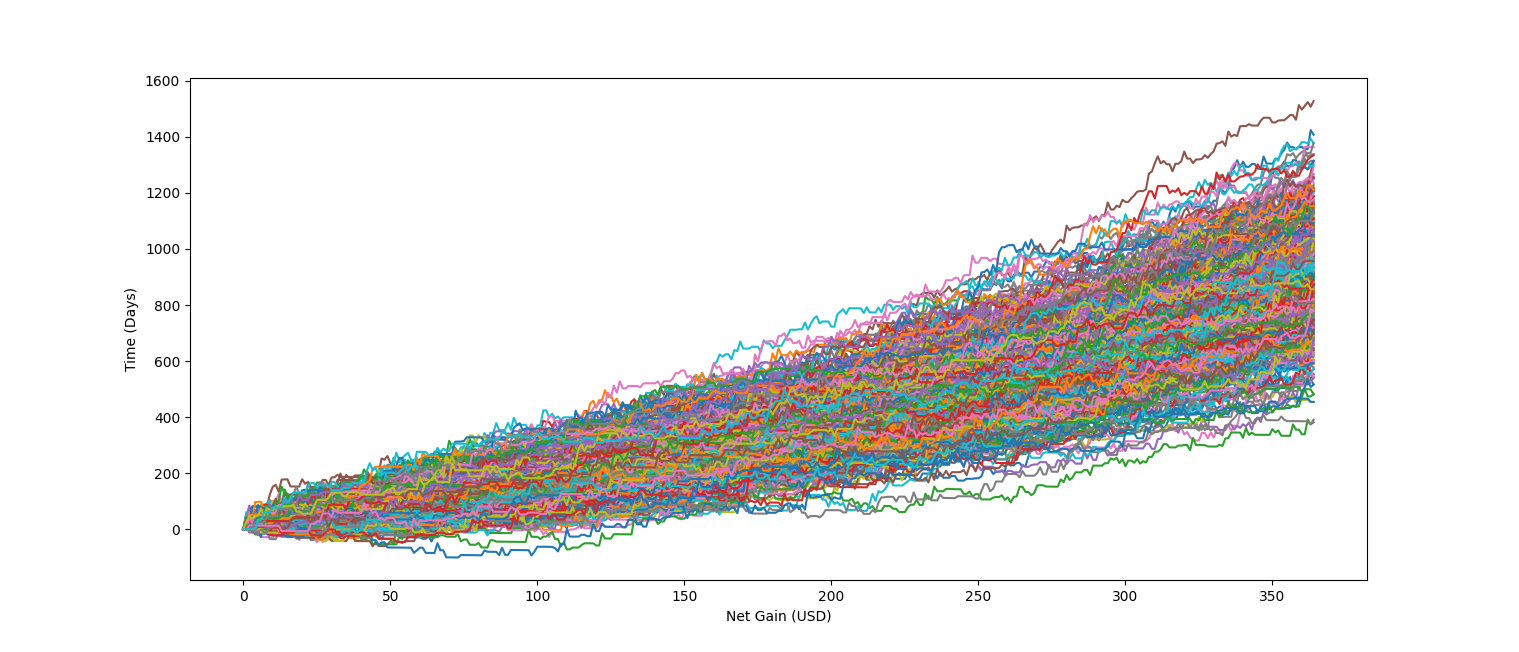
\includegraphics[scale=0.45]{monte-carlo.png}
        \end{center}

        Here are the results for income, expenses, and profit on average:

        \begin{lstlisting}
            Average Income: 3570.86
            Average Expenses: 2645.23
            Average Profit: 925.63 (25.921800582724018%)
        \end{lstlisting}
\end{enumerate}

\end{document}
